\documentclass[10pt]{beamer}
\usetheme{Madrid}
\usecolortheme{whale}
\setbeamertemplate{footline}[page number]
\setlength{\parindent}{0.6cm}

\usepackage[utf8]{inputenc}
\usepackage[spanish]{babel}
\usepackage{amsfonts}
\usepackage{amsmath}
\usepackage{amssymb}
\usepackage{graphicx}
\usepackage{booktabs}
\usepackage{tikz} 
\usepackage{subcaption}

% --- Información de la Portada ---
\title{Diseño de un Oscilador Local basado en PLL para Receptor de Banda Marina VHF}
\author[Grupo 4]{Dávila Tomassi, Carlos Valentino\\ Mendes Rosa, Agustín\\ Monja, Ernesto Joaquín}
\institute[UNC]{Universidad Nacional de Córdoba\\ Facultad de Ciencias Exactas, Físicas y Naturales}
\date{10 de junio de 2026}

\begin{document}

\begin{frame}
    \begin{tikzpicture}[remember picture,overlay]
        \node[opacity=0.2,anchor=center] at (current page.center) 
            {
\includegraphics[width=0.9\paperwidth]{Figuras/decoracion_a.png}};
    \end{tikzpicture}
    
    \titlepage
    \begin{center}
        \vspace{-0.5cm}
        
\includegraphics[width=6cm]{Figuras/unc_fcefyn_logo.png}
    \end{center}
    
\end{frame}

%-----------------------------------------------
\begin{frame}{Introducción}

En esta presentación se abordará el diseño de un oscilador local basado en un sistema \textit{Phase-Locked Loop} (PLL) y la selección de un mezclador (o \textit{mixer}) para el \textit{Down Converter} de un receptor de radio operando en la banda marina VHF.

\vspace{0.2cm}

Se explicitarán los siguientes puntos:

\vspace{0.2cm}

\begin{itemize}
    \item \textbf{Especificaciones del servicio:} Rango de frecuencias de operación y ancho de canal de la banda elegida.
    \item \textbf{Cálculos del sistema PLL:} Tabla de valores de los divisores (prescaler) y cálculo de los componentes del filtro de lazo.
    \item \textbf{Selección de componentes:} Criterios adoptados para cada etapa del oscilador.
    \item \textbf{Selección del mezclador:} Selección basada en las frecuencias, niveles de señal esperados en el receptor y las ganancias necesarias de LO y RF.
\end{itemize}

\end{frame}

%-----------------------------------------------
\begin{frame}{Marco Teórico}
    \begin{itemize}
        \item \textbf{Receptor Superheterodino:} La señal entrante de RF se acondiciona y se desplaza a una Frecuencia Intermedia (FI) fija y más baja mediante un proceso de batido efectuado en el mezclador, facilitando el filtrado y la demodulación.
    \end{itemize}

        \begin{figure}
            \centering
            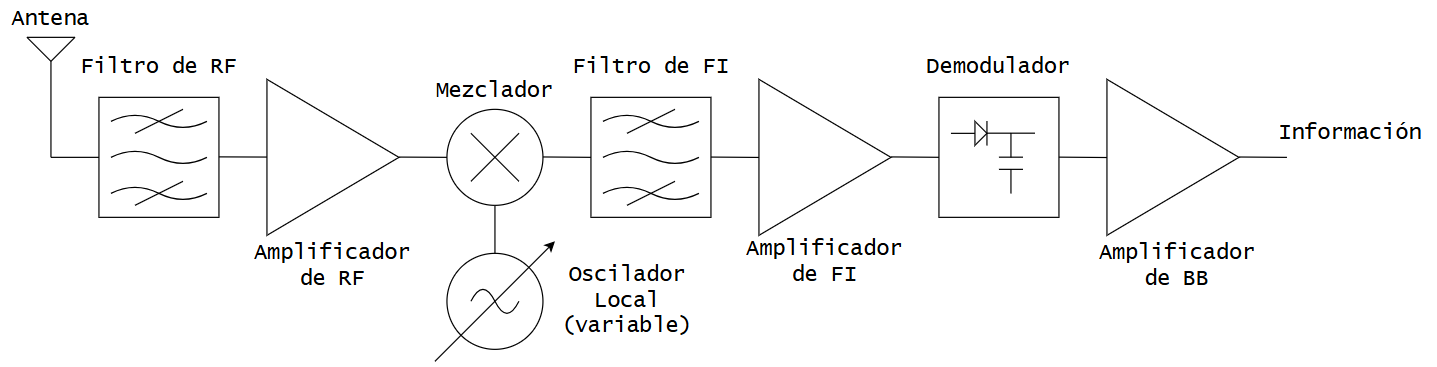
\includegraphics[width=0.8\linewidth]{Figuras/fig_superheterodino.png}
        \end{figure}
        
    \begin{itemize}
        \item \textbf{El Mezclador:} Componente no lineal que multiplica la señal de RF por la del Oscilador Local ($f_{LO}$) para obtener la componente de FI:
        $$f_{FI} = |f_{RF} \pm f_{LO}|$$
        
        Para lograr esta igualdad, es necesario diseñar el oscilador local tal que se cumpla:
        $$f_{LO} = f_{RF} \pm f_{FI}$$
    \end{itemize}
\end{frame}

%-----------------------------------------------
\begin{frame}{Marco Teórico}
    
    \begin{itemize}        
        \item \textbf{Oscilador Local con PLL:} Se parte de un \textit{Voltage-Controlled Oscillator} (VCO) que otorga variabilidad. Éste se realimenta comparándolo con una referencia de alta precisión mediante un detector de fase, que envía un valor de tensión según la diferencia de fase entre dos señales. Se incorporan divisores en los bloques, tal que al variar su valor se cambia de canal de forma exacta.
    \end{itemize}
    
    \begin{figure}
        \centering
        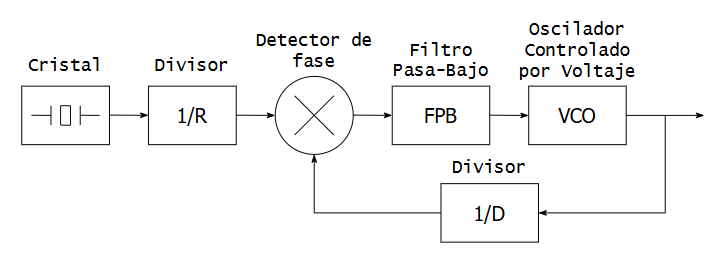
\includegraphics[width=0.8\linewidth]{Figuras/fig_PLL.png}
    \end{figure}
\end{frame}

%-----------------------------------------------
\begin{frame}{Elección del Servicio: Banda Marina VHF}
    \begin{block}{Servicio Elegido}
        Comunicación para Móvil Marítimo en la banda de VHF.
    \end{block}
    
    \vspace{0.3cm}
    
    \textbf{Aplicaciones Principales:}
    \begin{itemize}
        \item Coordinación operativa entre buques y estaciones costeras/portuarias.
        
        \item Operaciones críticas de seguridad, búsqueda y rescate (SAR) en el mar.

        \item Canal 16: Llamada de emergencia (obligatorio de escucha para todas las estaciones embarcadas y costeras).
    \end{itemize}

    \vspace{0.3cm}

    La banda marítima VHF abarca entre 156~MHz y 174~MHz según la ITU, con canales establecidos de 25~kHz \cite{uit}.
    
    Sin embargo, al no especificarse uso en la banda de 162~MHz a 174~MHz, el CABFRA dispuso esa banda para parte del Servicio Móvil Terrestre de Argentina, además de que se pierde la canalización fija de 25~kHz \cite{cabfra}. Debido a esto se plantea acotar la banda de trabajo de 156~MHz a 162~MHz.
    
\end{frame}

%-----------------------------------------------
\begin{frame}{Características Técnicas del Espectro (Acotado)}

    Según la tabla de frecuencias de la banda marina \cite{tabla_frec}, el primer canal activo (01) opera en $156.050\text{ MHz}$, mientras que el último canal asignado (88) lo hace en $162.025\text{ MHz}$. Por lo tanto, los límites del diseño se ajustarán a estos valores reales.

    \begin{exampleblock}{Parámetros de Diseño}
        \begin{itemize}
            \item \textbf{Rango de RF bajo análisis:} $156.050\text{ MHz}$ a $162.025\text{ MHz}$.
            \item \textbf{Ancho de Canal:} $\Delta f = 25\text{ kHz}$.
            \item \textbf{Frecuencia Intermedia (FI):} Seleccionada en $10.7\text{ MHz}$ (Estándar de VHF).
        \end{itemize}
    \end{exampleblock}

    \vspace{0.2cm}
    
    \textbf{Rango del Oscilador Local ($f_{LO}$)} con high-side tuning:
    $$f_{LO} = f_{RF} + f_{FI}$$
    \begin{itemize}
        \item $f_{LO(min)} = 156.050\text{ MHz} + 10.7\text{ MHz} = 166.750\text{ MHz}$
        \item $f_{LO(max)} = 162.025\text{ MHz} + 10.7\text{ MHz} = 172.725\text{ MHz}$
    \end{itemize}
\end{frame}

%-----------------------------------------------
\begin{frame}{Cálculo de la Tabla de Divisores del PLL}

    Los valores extremos del factor de división $D$, si se usa un clock de $f_{ref} = \Delta f$ del canal, se obtienen según:
    $$D_{min} = \frac{f_{LO(min)}}{f_{ref}} = \frac{166,750~MHz}{25~kHz} = 6670$$

    
    $$D_{max} = \frac{f_{LO(max)}}{f_{ref}} = \frac{172,725~MHz}{25~kHz} = 6909$$

    \vspace{0.2 cm}

    Dado $D_{min}$, se obtiene el módulo para el prescaler ($N$):
    $$D_{min} \geq N(N-1) \xrightarrow{} N = 64$$

    \vspace{0.2 cm}
    
    Tal que, si se usa un divisor de Doble Módulo, se cumple la siguiente igualdad:
    $$D = B \cdot N + A$$
    
\end{frame}

%-----------------------------------------------
\begin{frame}{Cálculo de la Tabla de Divisores del PLL}
    Se utilizará entonces un divisor de Doble Módulo 64/65, logrando así:
    
    \vspace{0.3 cm}

    \textbf{1. Para el Canal Mínimo} ($f_{LO(min)} = 166.750\text{ MHz}$):
    \begin{itemize}
        \item $D_{min} = 6670$
        \item $B_{min} = \frac{6670}{64} = 104,21 \xrightarrow{} 104$
        \item $A_{min} = 6670 - (104 \cdot 64) = 14$
    \end{itemize}

    \vspace{0.3 cm}
    
    \textbf{2. Para el Canal Máximo} ($f_{LO(max)} = 172.725\text{ MHz}$):
    \begin{itemize}
        \item $D_{max} = 6909$
        \item $B_{max} = \frac{6909}{64} = 107,95 \xrightarrow{} 107$
        \item $A_{max} = 6909 - (107 \cdot 64) = 61$
    \end{itemize}
\end{frame}

%-----------------------------------------------
\begin{frame}{Tabla de Frecuencias Sintonizables}
    \begin{figure}
        \centering
        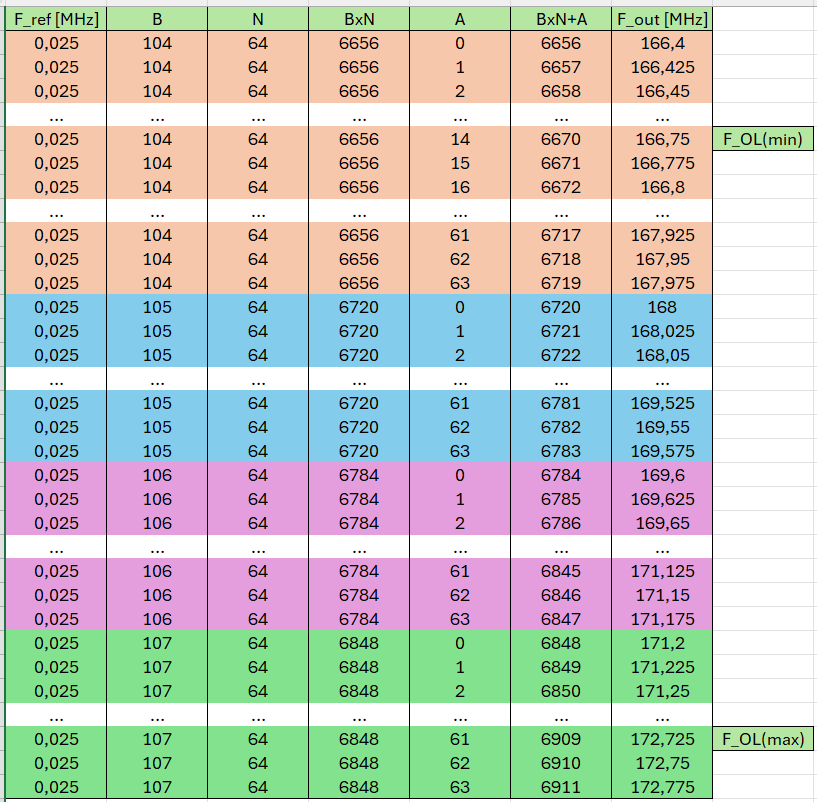
\includegraphics[width=0.65\linewidth]{Figuras/fig_tabla.png}
    \end{figure}
\end{frame}

%-----------------------------------------------
\begin{frame}{Selección del Divisor de Doble Módulo}

    Se selecciona el prescaler \textbf{Motorola MC12028A} bajo un estricto criterio de compatibilidad y eficiencia energética \cite{mc12028a}:

    \vspace{0.2cm}
    \begin{itemize}
        \item \textbf{Módulo:} Permite seleccionar el módulo $64/65$ requerido para el diseño.
        \item \textbf{Menor Consumo:} Posee un consumo típico de $4.0\text{ mA}$, reduciendo a la mitad el consumo frente a opciones como el MB501L ($\sim 10\text{ mA}$).
        \item \textbf{Ancho de Banda:} Posee una frecuencia máxima de trabajo de $1.1$ GHz, por lo que trabajará correctamente con la señal del VCO.
    \end{itemize}

    \begin{figure}
    \centering
    \begin{subfigure}{0.3\linewidth}
        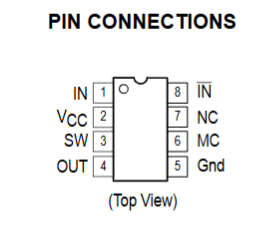
\includegraphics[width=\linewidth]{Figuras/fig_mc1.png}
    \end{subfigure}
    \hspace{0.1 cm}
    \begin{subfigure}{0.4\linewidth}
        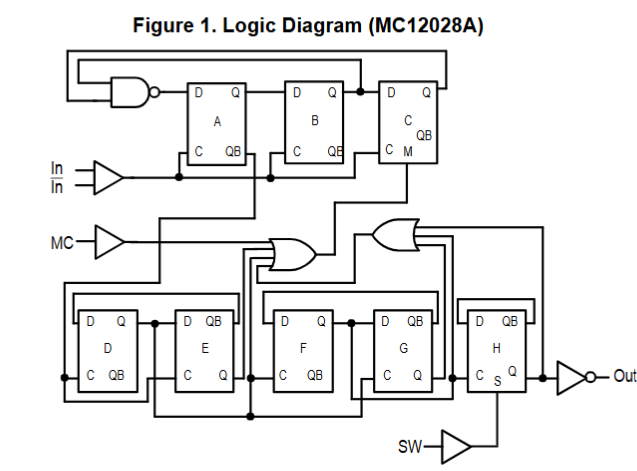
\includegraphics[width=\linewidth]{Figuras/fig_mc2.png}
    \end{subfigure}
    \end{figure}
\end{frame}

%-----------------------------------------------
\begin{frame}{Selección del Detector de Fase}

Se selecciona el \textbf{Motorola MC4044}, un detector de fase y frecuencia (PFD), que entrega un valor de tensión de error proporcionales al desfasaje entre dos señales de entrada \cite{mc4044}. Se escoge al ser un bloque dedicado, contiene los detectores lógicos evitando componentes o subcircuitos en la placa.

Es necesario determinar la ganancia $K_D$, por lo que teniendo en cuenta que el componente se comporta según:
$$V_{dc} = K_D(\phi_{2} - \phi_1)$$

    \begin{figure}
        \centering
        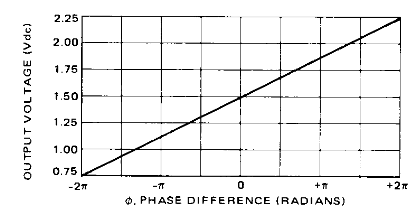
\includegraphics[width=0.4\linewidth]{Figuras/fig_KD.png}
    \end{figure}
    
    Observándose una función lineal, puede determinarse el siguiente valor:
    $$K_D = \frac{\Delta V_{dc}}{\Delta \phi} = \frac{2.25 - 0.75}{2 \pi - (-2 \pi)} = 0,119 \ \frac{V}{rad}$$
\end{frame}

%-----------------------------------------------
\begin{frame}{Selección del VCO}

Se selecciona el módulo comercial \textbf{Mini-Circuits ROS-200-619+} \cite{ros200}:

    \vspace{0.2cm}
    \begin{itemize}
        \item \textbf{Cobertura de Banda:} Opera entre $155\text{ MHz}$ y $200\text{ MHz}$, abarcando completamente la banda de Oscilador Local ($166.75\text{ MHz}$ a $172.725\text{ MHz}$).
        \item \textbf{Rango de Entrada:} Para los extremos de la banda, las tensiones de entrada se extienden de $1,77$ V a $2,17$ V, ideal para la salida del MC4044.
    \end{itemize}

    \begin{figure}
        \centering
        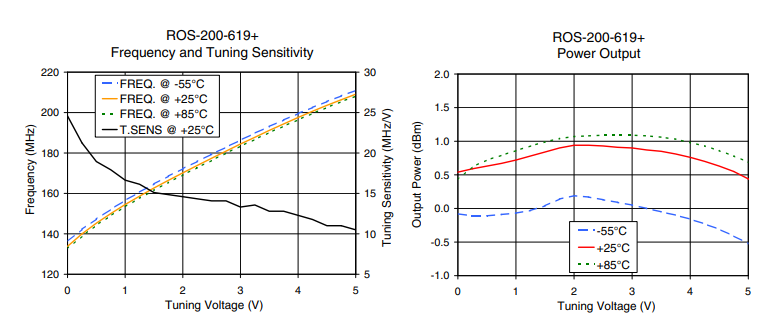
\includegraphics[width=0.7\linewidth]{Figuras/fig_VCO.png}
    \end{figure}

Para la banda de interés, la ganancia del VCO puede estimarse:
$$K_{VCO} = \frac{\Delta f_{LO}}{\Delta V_{in}} = \frac{(172,725 - 166,75)MHz}{(2.17 - 1,77)V} = 14.9 \ \frac{MHz}{V} = 93.6\ \frac{Mrad}{s\cdot V}$$

\end{frame}

%-----------------------------------------------
\begin{frame}{Diseño de Filtro de Lazo}

Si se toma como entrada y salida las fases de las señales en el PLL, según el diagrama de bloques, la función de transferencia del sistema es:

$$F_T(s) = \frac{K_D \cdot F_{FPB}(s) \cdot K_{VCO}}{s + \frac{K_D \cdot F_{FPB}(s) \cdot K_{VCO}}{D}}$$

\vspace{0.2cm}
Se desea lograr un sistema de tipo 2, para obtener $e_{ss}$ de frecuencia nulo, por lo tanto, se implementa un FPB Activo Proporcional Integral \cite{ogata}:

\begin{figure}
    \centering
    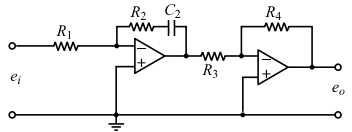
\includegraphics[width=0.4\linewidth]{Figuras/fig_PI.png}
\end{figure}


Determinando $R_3 = R_4$, su función de transferencia es:
$$F_{FPB}(s) = \frac{1 + s\tau_2}{s\tau_1}$$

Donde $\tau_1 = R_1 C_2$ y $\tau_2 = R_2 C_2$.


\end{frame}

%-----------------------------------------------
\begin{frame}{Diseño de Filtro de Lazo}

Reemplazando en la ecuación original,resulta:
$$F_T(s) = \frac{s \left(\frac{\tau_2 \cdot K_D \cdot K_{VCO}}{\tau_1}\right) + \left(\frac{K_D \cdot K_{VCO}}{\tau_1}\right)}{s^2 + \frac{s \cdot \tau_2 \cdot K_D \cdot K_{VCO}}{\tau_1 \cdot D} + \frac{K_D \cdot K_{VCO}}{\tau_1 \cdot D}}$$

Comparando con el denominador de la forma canónica de un sistema de 2do orden ($s^2 + 2\zeta \omega_ns + \omega_n^2$), se deducen los parámetros:

$$ \omega_n = \sqrt{\frac{K_D \cdot K_{VCO}}{\tau_1 \cdot D}} \quad \text{;} \quad \zeta = \frac{\tau_2 \cdot \omega_n}{2} \quad \text{;} \quad K_0 = D$$

\vspace{0.2 cm}

La frecuencia de corte ($f_n$) del sistema se plantea 50 veces menor a la $f_{ref} = 25~kHz$ para asegurar el filtrado de la misma, y se elige $\zeta$ para amortiguamiento crítico. Por lo tanto se adoptan los siguientes parámetros:
\begin{itemize}
    \item $\omega_n = 2\pi \cdot f_n = 2\pi \cdot 500 = 3141.6\text{ rad/s}$.
    \item $\zeta = 0.707$ 
\end{itemize}
\end{frame}

%-----------------------------------------------
\begin{frame}{Diseño de Filtro de Lazo}
    
Tomando $D = D_{prom} = 6789.5$ y reemplazando los valores de las ganancias correspondientes, resulta:

$$ \tau_1 = \frac{K_D \cdot K_{VCO}}{D \cdot \omega_n^2} = \frac{0,119 \cdot 93,6 \cdot 10^6}{6789,5 \cdot (3141,6)^2} =166,2\text{ }\mu\text{s} = R_1 \cdot C$$

$$ \tau_2 = \frac{2 \cdot \zeta}{\omega_n} = \frac{2 \cdot 0.707}{3141,6} = 450\text{ }\mu\text{s} = R_2 \cdot C$$

\vspace{0.2 cm}

Se asume un capacitor comercial de $C = 100\text{ nF}$ y se obtiene:

$$ R_1 = \frac{\tau_1}{C} = \frac{166,2 \cdot 10^{-6}}{100 \cdot 10^{-9}} = 1662 \ \Omega$$

$$ R_2 = \frac{\tau_2}{C} = \frac{450 \cdot 10^{-6}}{100 \cdot 10^{-9}} = 4500 \ \Omega$$

\end{frame}

%-----------------------------------------------
\begin{frame}{Diseño de Filtro de Lazo}
    
Por último, la elección del chip del operacional para el filtro es el \textbf{Texas Instruments TL072} \cite{opamp}:

\vspace{0.2cm}
\begin{itemize}
    \item \textbf{Corriente de Polarización Baja:} Gracias a sus entradas JFET, presenta una corriente de fuga típica de 65 pA.
    \item \textbf{Slew Rate:} Tasa de crecimiento suficiente para trabajar con frecuencias de los kHz de forma estable.
    \item \textbf{Encapsulado Dual:} Al disponer de dos amplificadores, con un solo chip es suficiente para abarcar los operacionales del filtro.
\end{itemize}

\end{frame}

%-----------------------------------------------
\begin{frame}{Selección del Mezclador}

Se adoptará un mezclador de modelo \textbf{ADE-6+} de Mini-Circuits \cite{ad6}:

\vspace{0.1cm}
\begin{itemize}
    \item \textbf{Frecuencias:} Soporta la entrada de RF ($156,05-162,025\text{ MHz}$), la inyección de LO ($166,75-172,725\text{ MHz}$) y la extracción de FI ($10,7\text{ MHz}$).
    
    \item \textbf{Niveles de Señal de RF:} Evaluando el peor caso, con Tx de 25~W = 44~dBm, a 0.1~km en 160~MHz, la atenuación de espacio libre \cite{fspl} es:
    $$FSPL = 20 \log_{10}(0,1) + 20 \log_{10}(160) + 32,44 \approx 56,5\text{ dB}$$
    La señal recibida máxima será de -12,5~dBm. Al ser mucho menor al Punto de Compresión (1~dBm), el mezclador trabajará siempre en su región lineal.

    \item \textbf{Nivel del Oscilador Local:} Dado que el VCO entrega entre 0.5 y 1~dBm, se incorporará un amplificador con ganancia de 7 dB antes de entrar al mixer y cumplir con el LO level de 7~dBm.
    
\end{itemize}



\end{frame}

%-----------------------------------------------
\begin{frame}{Selección del Mezclador}
\begin{itemize}
    \item \textbf{Pérdida de Conversión (Conversion Loss):} Presenta el menor valor de $4,6\text{ dB}$ frente a los otros modelo que cumplían requisitos preliminares.
    \item \textbf{Aislamiento (Isolation):} Posee una atenuación típica de 40 dB tanto entre los puertos LO-RF como LO-FI, bloqueando la filtración del oscilador local hacia la antena o hacia las etapas posteriores de FI.
\end{itemize}

\vspace{0.3cm}
\begin{block}{Rango Dinámico y Regla de Operación}
    El diseño cumple la recomendación de que $P_{LO} \ge P_{RF} + 10\text{ dB}$. Al inyectar $7\text{ dBm}$ de LO frente a una señal máxima extrema de RF de $-12,5\text{ dBm}$, el oscilador local controla la conmutación de los dispositivos y obtiene mejor eliminación de intermodulaciones.
\end{block}
\end{frame}

%-----------------------------------------------
\begin{frame}[allowframebreaks]{Bibliografía y Referencias}
    \begin{thebibliography}{9}

        \bibitem{apunte_catedra} 
        Dadam, F; Bruni, R. \textit{Apunte de Cátedra. Electrónica Analógica III.}
        \\ {\scriptsize FCEFyN, Universidad Nacional de Córdoba (2026).}

        \vspace{0.1 cm}

        \bibitem{uit} 
        International Telecommunication Union (ITU).
        \textit{Reglamento de Radiocomunicaciones, Apéndice 18}. 
        \\ {\scriptsize \url{https://search.itu.int/history/HistoryDigitalCollectionDocLibrary/4.125.81.en.1000.pdf}}

        \vspace{0.1 cm}

        \bibitem{cabfra} 
        Ente Nacional de Comunicaciones (ENACOM). 
        \textit{Cuadro de Atribución de Bandas de Frecuencias de la República Argentina (CABFRA)}.
        \\ {\scriptsize \url{https://www.enacom.gob.ar/cuadro-de-atribucion-de-bandas-de-frecuencias-de-la-republica-argentina-cabfra-_p1588}}

        \vspace{0.1 cm}

        \bibitem{tabla_frec} 
        Tabla de frecuencias canales marinos.
        \\ {\scriptsize \url{https://www.radioservice.com.ar/canales_marinos.html}}
        
        \vspace{0.1 cm}

        \bibitem{mc12028a} 
        Motorola MC120228A. \textit{Hoja de datos.}
        \\ {\scriptsize \url{https://www.alldatasheet.com/datasheet-pdf/view/898197/MOTOROLA/MC120228BP.html}}

        \vspace{0.1 cm}

        \bibitem{mc4044} 
        Motorola MC4044. \textit{Hoja de datos.}
        \\ {\scriptsize \url{https://www.alldatasheet.es/datasheet-pdf/view/86788/MOTOROLA/MC4044.html}}

        \vspace{0.1 cm}

        \bibitem{ros200} 
        Mini-Circuits ROS-200-619+. \textit{Hoja de datos.}
        \\ {\scriptsize \url{https://www.minicircuits.com/pdfs/ROS-200-619+.pdf}}

        \vspace{0.1 cm}

        \bibitem{ogata} 
        Ogata, Katsuhiko. \textit{Ingeniería de Control Moderna. 5ta edición. Página 85.}
        \\ {\scriptsize \url{https://ingenierovizcaino.com/material/libros/sd/ingenieria-de-control-moderna-ogata-5ed.pdf}}

        \vspace{0.1 cm}

        \bibitem{opamp} 
        Texas Instruments TL072. \textit{Hoja de datos.}
        \\ {\scriptsize \url{https://www.alldatasheet.com/datasheet-pdf/view/28775/TI/TL072.html}}

        \vspace{0.1 cm}

        \bibitem{fspl} 
        Cadence PCB Education. \textit{Free-Space Path Loss.}
        \\ {\scriptsize \url{https://resources.pcb.cadence.com/blog/2024-free-space-path-loss}}

        \vspace{0.1 cm}

        \bibitem{ad6} 
        Mini-Circuits ADE-6+. \textit{Hoja de datos.}
        \\ {\scriptsize \url{https://www.minicircuits.com/pdfs/ADE-6+.pdf}}
        
    \end{thebibliography}
\end{frame}

\end{document}